\documentclass[12pt]{article}
\usepackage{graphicx}
\begin{document}
\title{Document Tender}

\begin{titlepage}
\begin{huge}
\begin{center}
Project Tender

Project: Swarm Visualiser
\\
\begin{LARGE}
Client: Christopher Cleghorn
\end{LARGE}

Team: Dragon Brain
\\
\begin{small}
Department of Computer Science, University of Pretoria
\\
\begin{itemize}
\item Matheu Botha u14284104
\item Renton McIntyre u14312710
\item Emilio Singh u14006512
\item Gerard van Wyk u14101263
\end{itemize}


Date: 2016/05/02

\end{small}

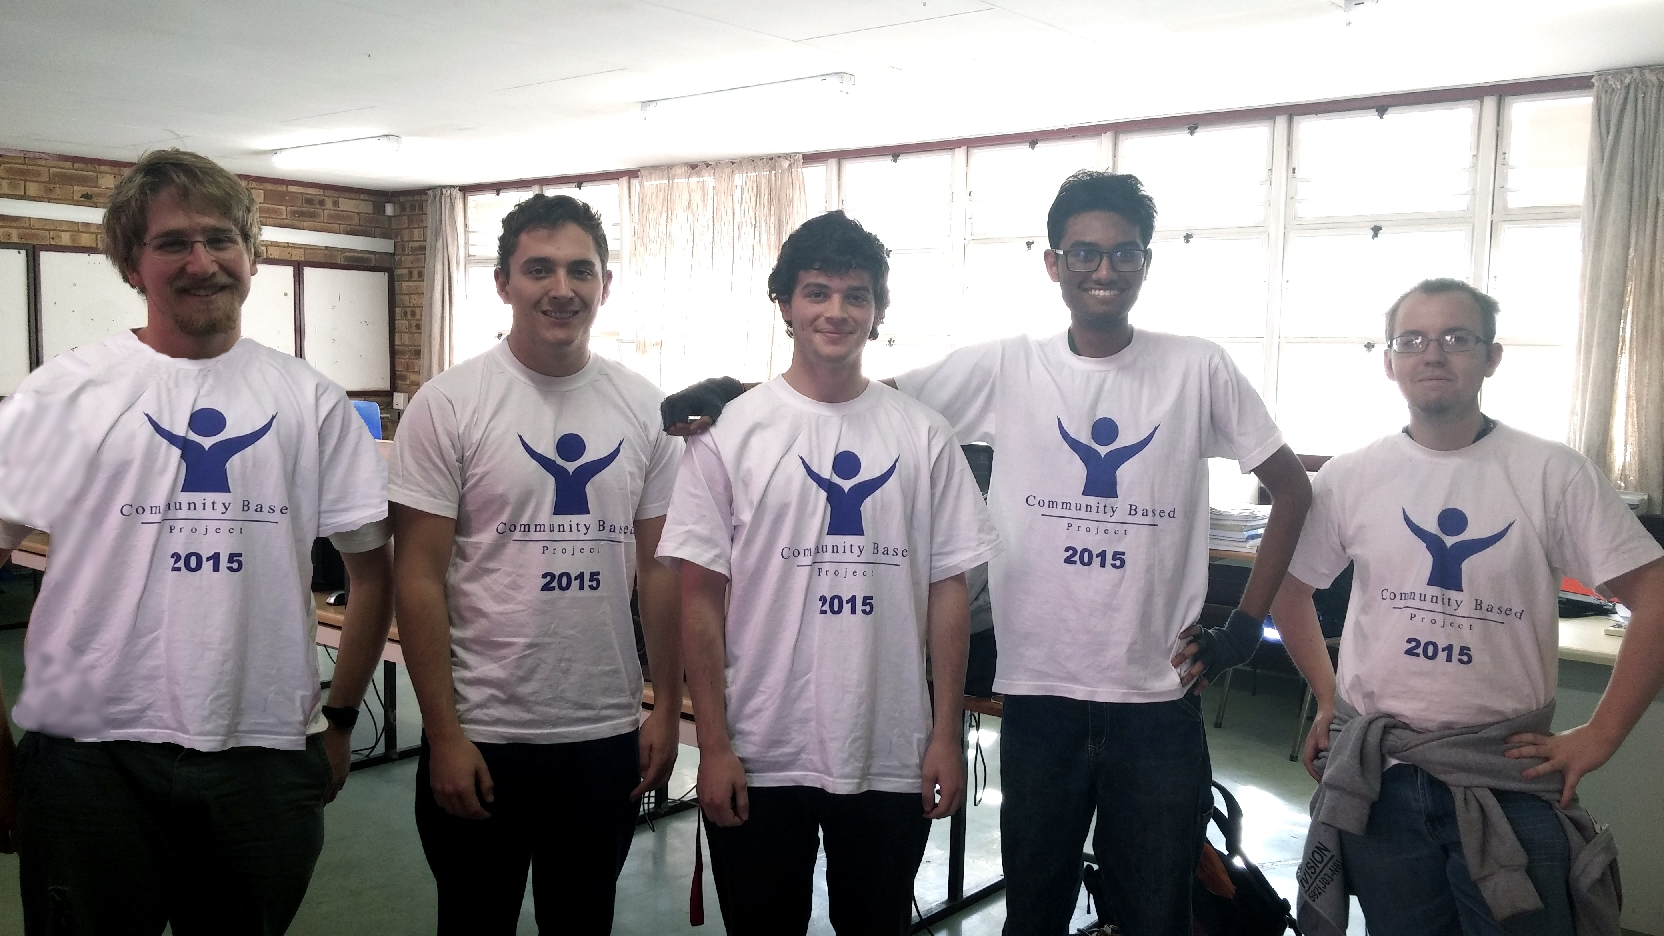
\includegraphics[scale=0.2]{JCPfinalPoseLowres}
\end{center}

\end{huge}


\end{titlepage}

\pagebreak

\section{The Team}
\subsection{Matheu Botha}
\includegraphics[scale=0.5]{Matheu.JPE}

\paragraph{Interests}
My main interests with regard to academia lie in Artificial Intelligence. However as a career path I have always been interested in is game development. This is because I believe that games are the most progressive form of art. They require , arguably, the most diverse skill set. It requires everything from programmatic knowledge to Human Computer Interaction(HCI). 

\paragraph{Technical Skills}
	I am proficient in the following programming languages:
	\begin{itemize}
		\item C++
		\item C\#
		\item Java
		\item Javascript
		\item Python
		\item PHP
	\end{itemize}

\paragraph{Relevant Past Experience}
	In the past I have done projects with Monkey and River developing the SALGA Municipal Barometer. I have also worked with Merlynn Intelligent Technologies developing the UP2TOM app. Both of these projects involved extensive Front End development which has given me experience with regard to developing User Interfaces, which is relevant for the project. I have also been working as a part time technical assistant for the university of Pretoria which has afforded me the opportunity to work with many enterprise level development technologies in a production environment.

\paragraph{Non-technical Strengths}
	I enjoy working as part of a team on a large project. I am also very challenge driven. I enjoying taking on challenging projects and working hard with a group of like minded individuals to overcome those challenges.

\paragraph{Motivation for Project}
	I would like to work on this project because it is a very progressive field that still has the potential for a lot of innovative work to be done in it. In addition to that, this project relates to the field of study that I intend to study towards after I have achieved my bachelors degree.

\subsection{Renton McIntyre}

\includegraphics[scale=0.25]{Renton}
\paragraph{Interests}
My relevant interests include the fields of Artificial Intelligence and general academic advancement and experimentation.
\paragraph{Technical Skills}
I have had prolonged exposure to Java and C++ (the latter of which I consider to be my primary language). I also have experience with various scripting languages, C and Assembly.

Otherwise, I have some mathematical prowess and, perhaps above all else, a proficiency in the ability to learn technical skills on short notice.
\paragraph{Relevant Past Experience}
I have very few past experience with such projects. However, I am willing to learn and believe I will be able to make a valuable contribution towards the project.

\paragraph{Non-technical Strengths}
I believe I have a strong capability to work with people and have previously shown my ability to maintain my connection with a team well, often from the perspective of serving as somewhat of an assistant to the person in charge, as I do not often take such a role myself, despite potentially having the capability. 
\newline I also believe I have a good ability to apply concepts to practicality.
\paragraph{Motivation for Project}
The suggested Particle Visualiser piques my interest on a variety of levels, with a strong reliance on the field of AI being taken to a more human level. I have always been fascinated by the idea of projects that have huge potential for problem solving in our academic field, as well as those that have the potential to help humans, both highly academic and those without such knowledge, to understand the nature of scientific concepts. The Particle Visualizer is a perfect example of a project with brings such concepts together.

\subsection{Emilio Singh}
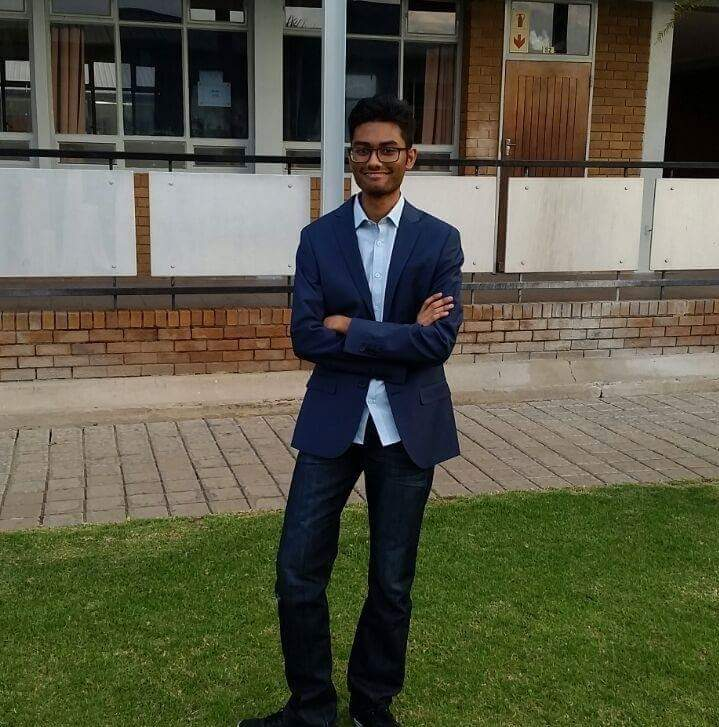
\includegraphics[scale=0.2]{Emilio}
\paragraph{Interests}
My relevant interests include the study of cryptography, video games and reading.
\paragraph{Technical Skills}
I can program using Java, C++, and a variety of scripting languages proficiently.
Furthermore, I have exposure, and somewhat fluency in Assembly.

My true strength would be in the field of mathematics and analysis however as I have shown high level competencies in various mathematical subjects while at university.
\paragraph{Relevant Past Experience}
Other than the 301 Mini Project, I have not worked on any major software system to this caliber but rest assured, I am very eager to learn and contribute towards the project.
\paragraph{Non-technical Strengths}
In terms of non-technical strengths, I would say that I have a capacity to serve in a leadership role. I have proven on numerous occasions that I can work with others and coordinate them towards a particular aim.

Furthermore, I feel that I have a level of skill with regards to communication with people from both technical and non-technical backgrounds which would typically aid in client-team communications.
\paragraph{Motivation for Project}
The Particle Visualiser Project combines very many of the topics that I feel particularly interested in especially with regards to field of swarm intelligence and how this relates to problem solving. The project offers me an excellent opportunity to work with these forms of technologies and issues in a format that cuts to the heart of the problem solving issue without descending to a more mundane commercial application.

Furthermore, I would also like to work on this project because I believe the client, Mr Cleghorn, would provide me not only with an excellent project to work on, but also provide a valuable learning experience into the field of swarm intelligence and optimisation.

\subsection{Gerard van Wyk}
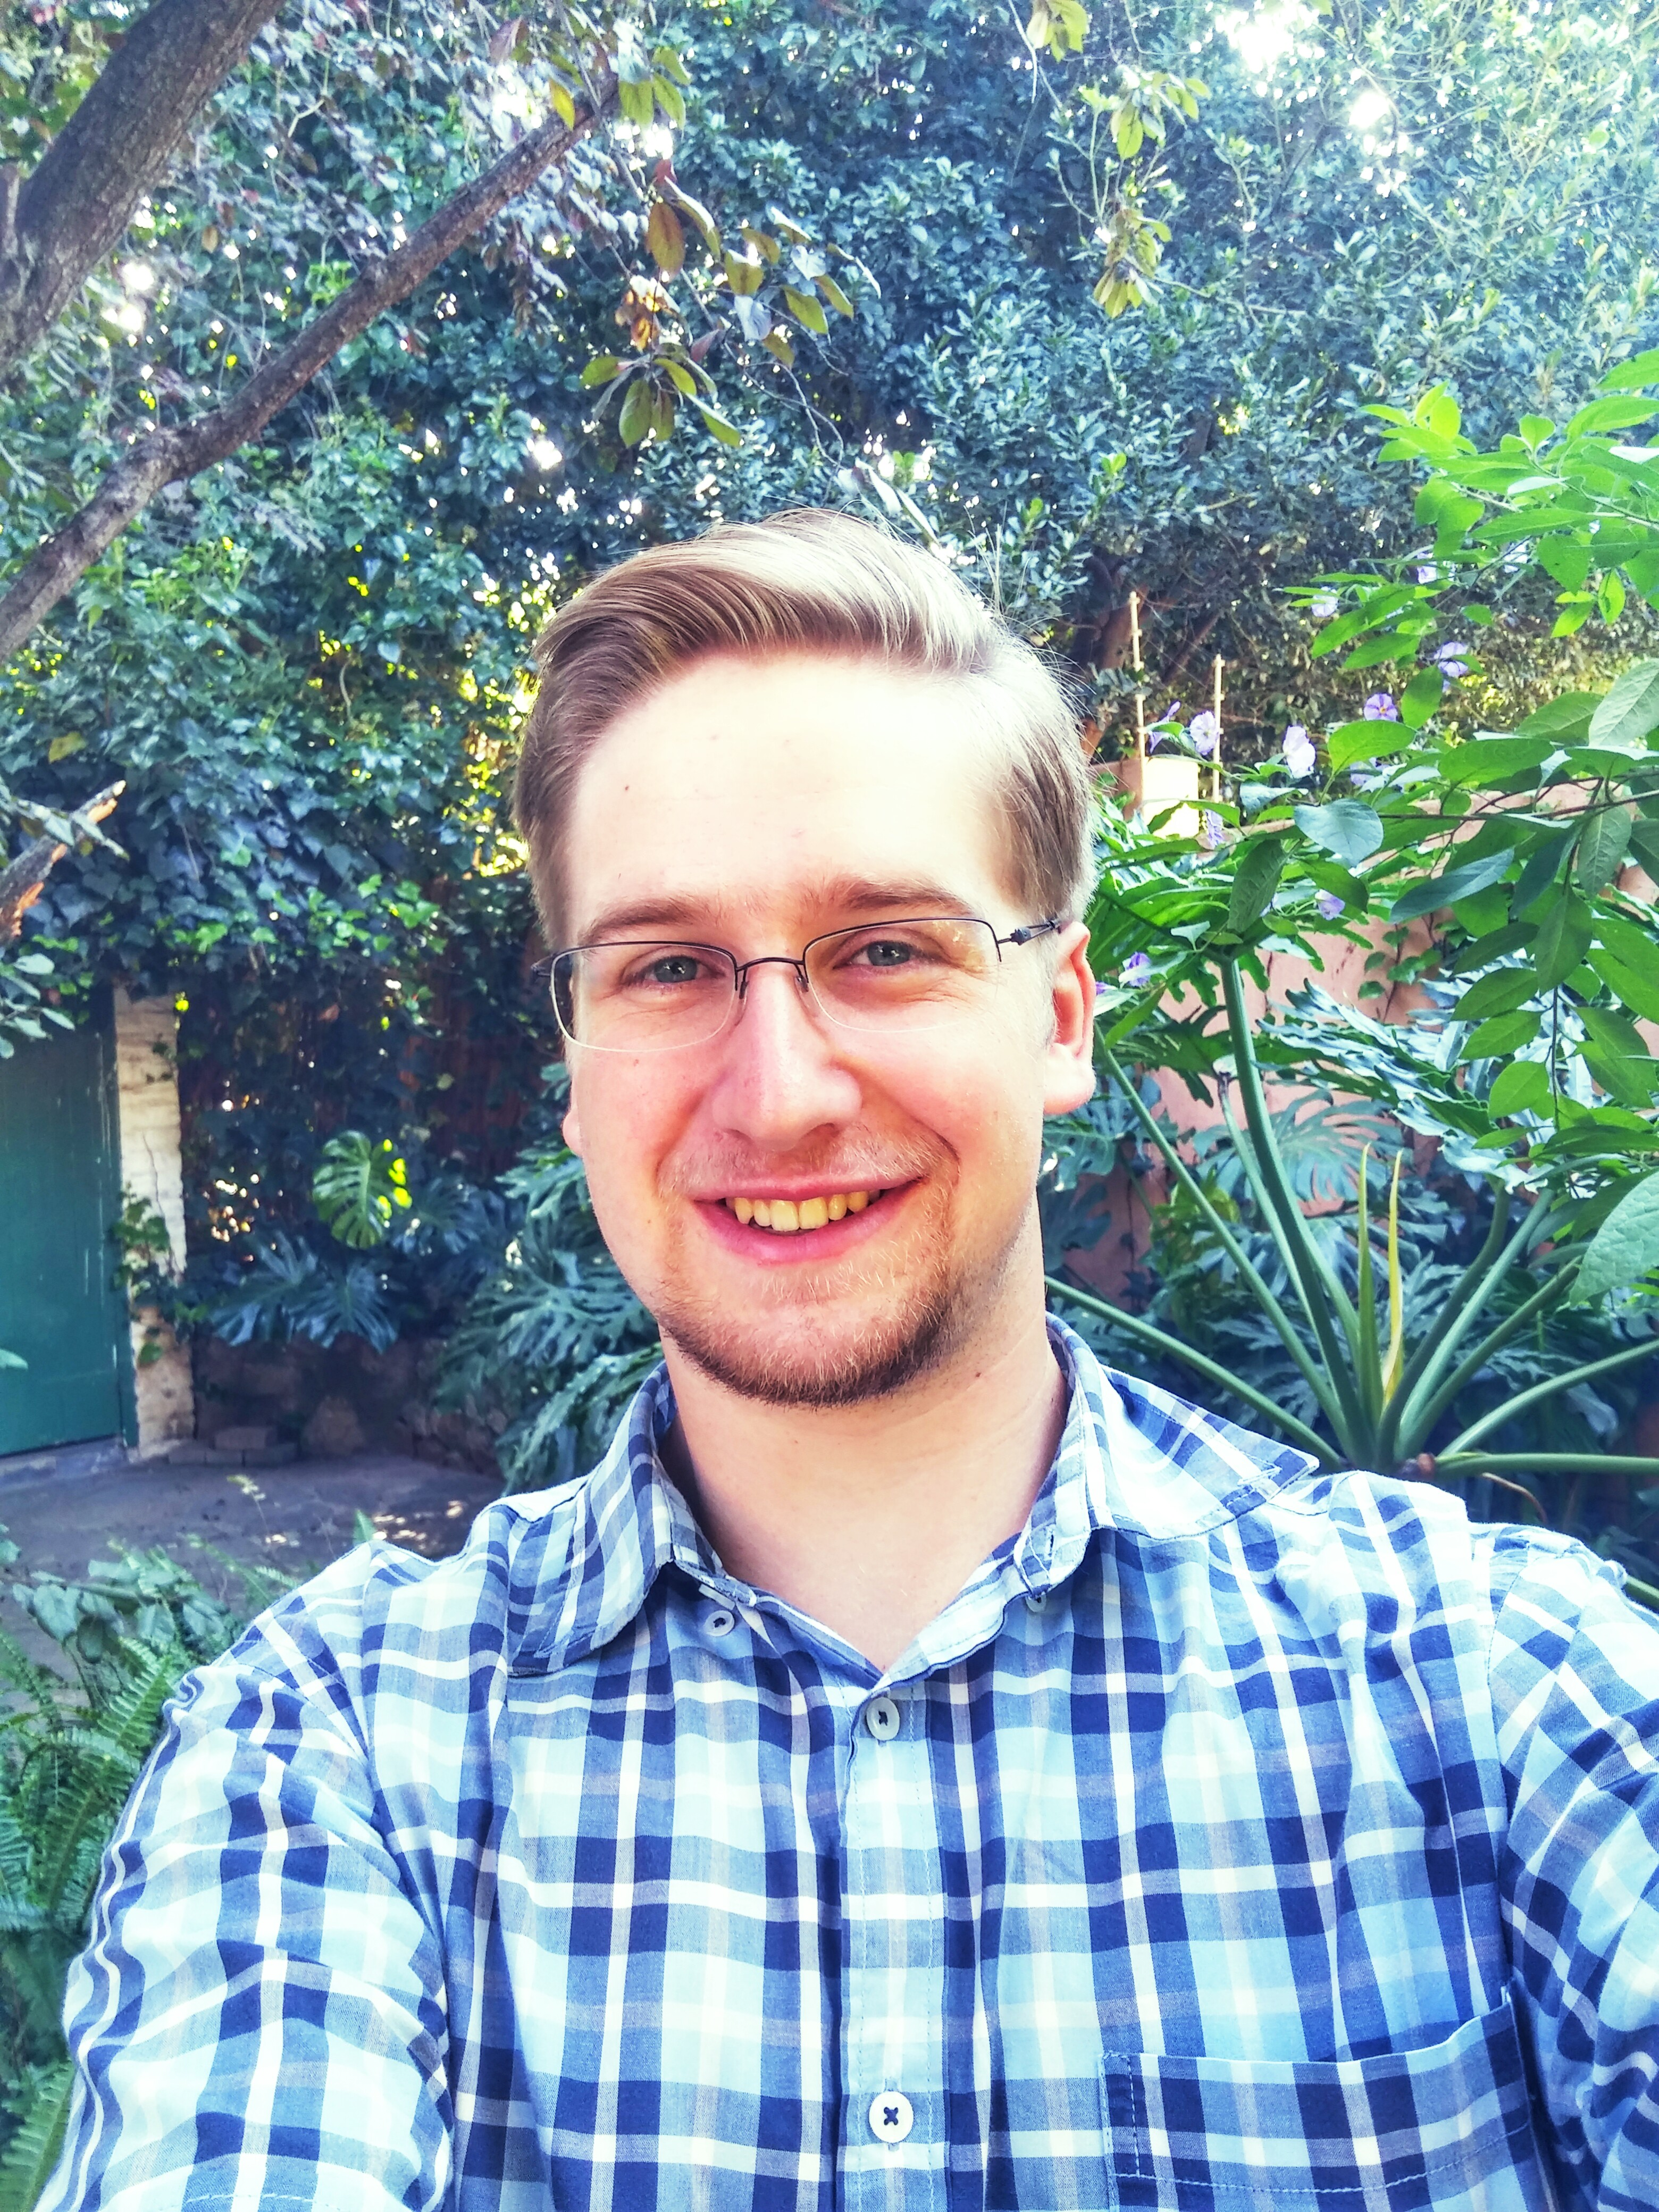
\includegraphics[scale=0.03]{Gerard}
\paragraph{Interests}
I am highly interested in Artificial Intelligence, video games/virtual reality and reading about science(especially space, geology and natural selection).
\paragraph{Technical Skills}
My programming language proficiencies are in Java, C++, and to a lesser extent OpenGL and general web languages.
Aside from programming languages: I am good at mathematics, and have a moderate skill in image and video editing.
\paragraph{Relevant Past Experience}
In the past I have built my own hillclimbing, simulated annealing, and genetic algorithms to tackle problems from shape packing to evolutionary programming. I believe I have a good understanding of the basics of locally searching through high-dimensional searchspaces, and understand the workings of many optimization algorithms.
\paragraph{Non-technical Strengths}
I work well with other people, learn quickly, am driven by intellectual curiosity, and always seek to achieve an efficient solution.
\paragraph{Motivation for Project}
Humans are primates optimized to live in a specific ecological niche in the African savannah, we possess great general learning capability but fall far short of completely understanding the increasingly abstract concepts that we invent in fields such as computer science. Teaching a human to code is like teaching someone without a visual cortex to draw, this is why we must invent tools to show abstract concepts such as optimization in a simple way - with colours, motion and a clear indication of success. This project is exactly that - a visualiser to show how optimization algorithms search through searchspaces in a manner we can easily understand. With such technology there is great potential to invent new algorithms, increase our understanding of old algorithms, and perhaps even make a part of the field of Artificial Intelligence less enigmatic to all.

\section{Project Execution}
\paragraph{Developmental Methodology}
We will be following an Agile development methodology. We hope to realise this development methodology by doing the following:
\begin{enumerate}
\item Communicating with our clients to ensure they are informed of project progress as well as to constantly refine and update our understanding of requirements in order to meet them.
\item Construct a frequent, working software delivery schedule so that incrementally working segments of the STORM project can be delivered to our clients.
\item Commit to the delivery of simplistic, maintainable and efficient software.
\item Accept that requirements for the project may change constantly throughout the project life-cycle and develop a modular system whose functioning can be easily adapted to suit this purpose.
\item We have a strong commitment to compartmentalisation of work and will adopt pair-programming and other team-oriented development practices as we are able to.

\end{enumerate}

\paragraph{Client-Team Communication Methods}
The client of this project is a member of the CS department. This means we have a definite means for on-site, face-to-face communications. We will coordinate with our client to make sure that we arrange our meetings within their schedule. Additionally, the option to email our client with additional requests outside of the normal operating hours also exists. Ideally however, we will endeavour to avail ourselves for our client as best we can.

Finally, we have also created a Slack group to manage the project team for the duration of the project. The clients will be extended the offer to join the group to be more directly related to intra-team communications.
\paragraph{Initial Ideas in response to Technical Challenges}
One of the technical challenges presented would the requirement that the systems runs at 60fps under the stated conditions. This means that we will have to run multiple benchmark tests on the system. To do this we can use a dependency injection to run a variety of unit tests on the system in a controlled environment.

Another technical challenge would be the fact that functions and algorithms need to be easy to add to the system. While it is simple enough to store a math function it is far more challenging to allow user defined algorithms. A potential solution would be for the system to have an api that a user could have their algorithm interact with.
\\
Furthermore, we would like to present a concept mock representing some of our initial ideas into what the project could look like when finalised. I would like to emphasize that this was done mostly out of enthusiasm on our part with regards to the project but as per Agile Development process, will more than likely come under revision as time goes on and requirements change.

\begin{figure}
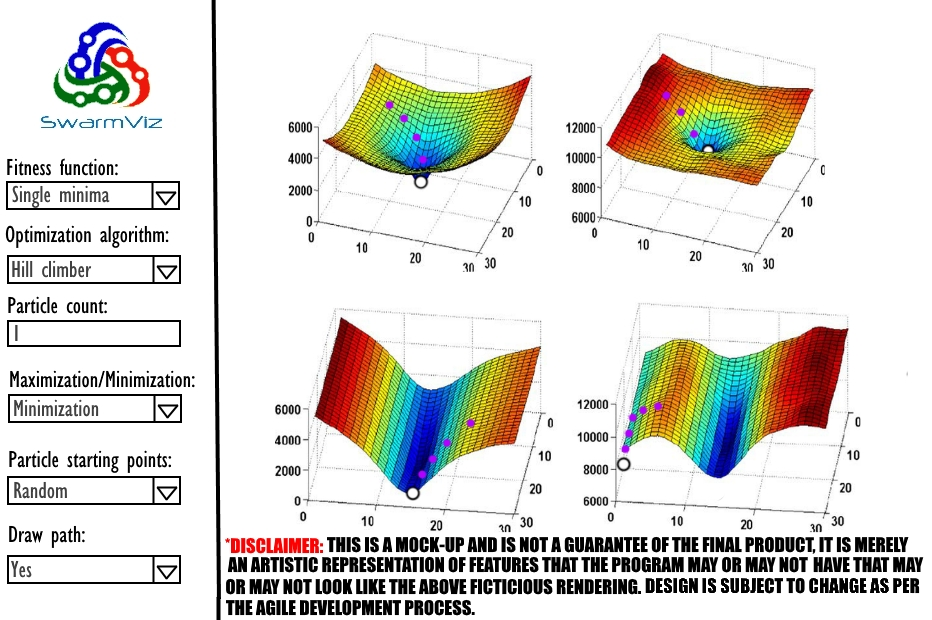
\includegraphics[scale=0.5]{SwarmVizMockup4}
\caption{A mockup to demonstrate a potential UI}
\end{figure} 

\pagebreak
\paragraph{Potential Technologies for use where not specified by client}
There are several potential frameworks that can be used for Dependency Injection, including:
\begin{itemize}
	\item Fruit
	\item Wallaroo
	\item Boost DI
\end{itemize}

\paragraph{Deliverable to Client}
The source code for the Swarm Visualiser will be handed over in the git repository. It is also possible for it to be compiled into an executable format. Possibly packaged into a virtual environment using a tool such as docker so that it can be deployed to a machine in a more contained manner. 
\end{document}
